%%%%%%%%%%%%%%%%%%%%%%%%%%%%%%%%%%%%%%%%%%%%%%%%%%%%%%%%
%%%%%%%%%%%%%%%%%%%% DOCUMENT BEGIN %%%%%%%%%%%%%%%%%%%%
%%%%%%%%%%%%%%%%%%%%%%%%%%%%%%%%%%%%%%%%%%%%%%%%%%%%%%%%

\documentclass[usenames,dvipsnames]{beamer}
%
% Choose how your presentation looks.
%
% For more themes, colour themes and font themes, see:
% http://deic.uab.es/~iblanes/beamer_gallery/index_by_theme.html
%
\mode<presentation>
{
  \usetheme{Warsaw}      % or try Darmstadt, Madrid, Warsaw, ...
  \usecolortheme{default} % or try albatross, beaver, crane, ...
  \usefonttheme{default}  % or try serif, structurebold, ...
  \setbeamertemplate{navigation symbols}{}
  \setbeamertemplate{caption}[numbered]
} 

\usepackage[english]{babel}
\usepackage[utf8x]{inputenc}
\usepackage{color}

\newtheorem{proposition}{Proposition}

% new commands for readability
\newcommand{\C}{\mathbb{C}}
\newcommand{\F}{\mathbb{F}}
\newcommand{\N}{\mathbb{N}}
\newcommand{\Q}{\mathbb{Q}}
\newcommand{\R}{\mathbb{R}}
\newcommand{\Z}{\mathbb{Z}}

\title[Groups Generated by Reflections]{Groups Generated by Reflections}
\author{Robert Lech}
\institute{Carleton University}
\date{\today}

\begin{document}

\begin{frame}
  \titlepage{}
\end{frame}

% Uncomment these lines for an automatically generated outline.
\begin{frame}{Outline}
 \tableofcontents
\end{frame}

%%%%%%%%%%%%%%%%%%%%%%%%%%%%%%%%%%%%%%%%%%%%%%%%%%%%%%%%
%%%%%%%%%%%%%%%%% INTRODUCTION BEGIN %%%%%%%%%%%%%%%%%%%
%%%%%%%%%%%%%%%%%%%%%%%%%%%%%%%%%%%%%%%%%%%%%%%%%%%%%%%%

\section{Introduction}

\subsection{Dihedral Groups}

\begin{frame}{Finite Dihedral Groups Generated by a Reflection and a Rotation}

Recall that finite dihedral groups, $D_n$, are commonly presented in terms of a rotation $r\in D_{n}$ and a
reflection $s\in D_{n}$. This can be seen as $D_{n}=<r,s|r^{n},s^{2},(rs)^{n}>$. This is seen below:

\begin{figure}[h]
    \label{fig:d5_rotations_reflections}
    \centering
    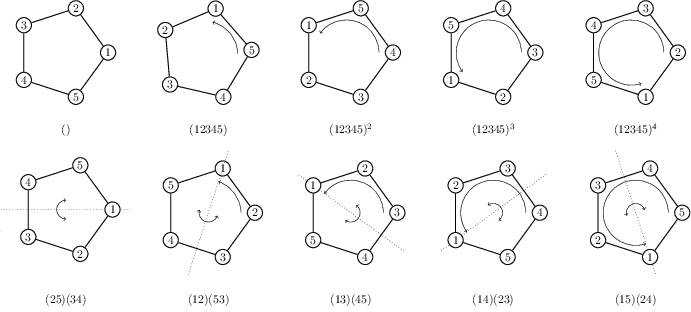
\includegraphics[width=0.70\textwidth]{images/d5_rotations_reflections.png}
    \caption{Rotations and Reflections of $D_5$}
\end{figure}

\end{frame}

\begin{frame}{Finite Dihedral Groups Generated by Reflections}

Also, recall that one can generate a finite dihedral group with two reflections $a,b\in D_n$. This is seen
below:

\pause{}

\begin{figure}[h]
    \centering
    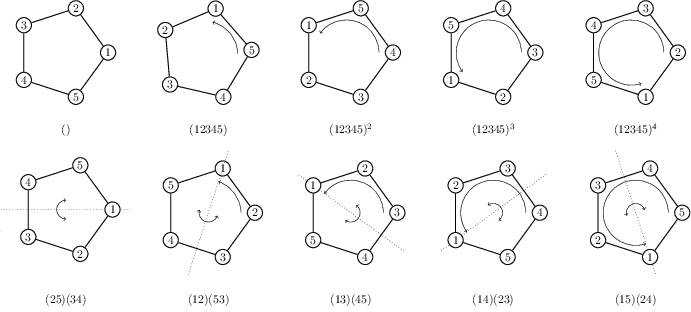
\includegraphics[width=0.50\textwidth]{images/d5_rotations_reflections.png}
    \caption{Rotations and Reflections of $D_5$}
\end{figure}

\end{frame}

\begin{frame}{Infinite Dihedral Groups}

\begin{itemize}
  \item Can we have a dihedral group with infinite elements?
  \pause{}
  \item How could you picture that?
  \pause{}
  \item What interesting things can we say about it?
\end{itemize}

\end{frame}

%%%%%%%%%%%%%%%%%%%%%%%%%%%%%%%%%%%%%%%%%%%%%%%%%%%%%%%%
%%%%%%% GROUPS GENERATED BY TWO REFLECTIONS BEGIN %%%%%%
%%%%%%%%%%%%%%%%%%%%%%%%%%%%%%%%%%%%%%%%%%%%%%%%%%%%%%%%

\section{Groups Generated by Two Reflections}

\begin{frame}{The Group Generated by 2 Reflections}

Suppose we looked at the Cartesian plane with two reflections defined: \textcolor{red}{$a[(x,y)]=(-x,y)$}
and \textcolor{blue}{$b[(x,y)]=(2-x,y)$}. The next few examples illustrates the orbit of
\textcolor{green}{$e$}.

\begin{figure}[h]
    \centering
    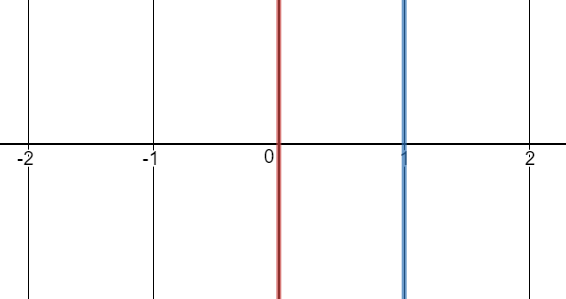
\includegraphics[width=0.50\textwidth]{images/1-01-d_inf.png}
    \caption{The axes of reflections $a$ and $b$.}
\end{figure}

\end{frame}

\begin{frame}{The Group Generated by 2 Reflections}

\begin{figure}[h]
    \centering
    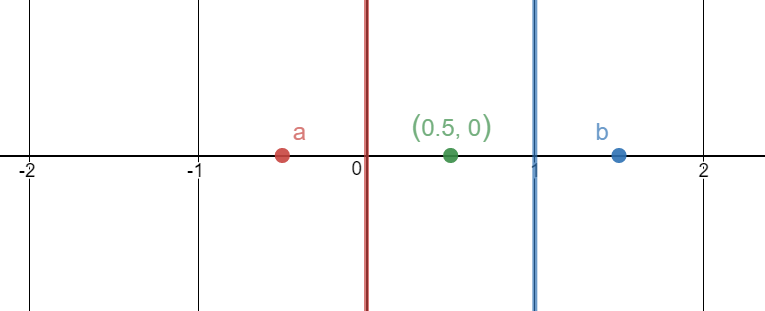
\includegraphics[width=1\textwidth]{images/1-02-d_inf_a_b.png}
    \caption{The images of $a[(0.5,0)]$ and $b[(0.5,0)]$.}
\end{figure}

\end{frame}

\begin{frame}{The Group Generated by 2 Reflections}

\begin{figure}[h]
    \centering
    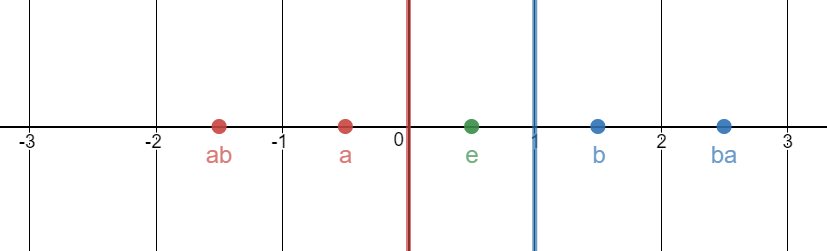
\includegraphics[width=1\textwidth]{images/1-04-d_inf_ab_1.png}
    \caption{The images of $ab[(0.5,0)]$ and $ba[(0.5,0)]$.}
\end{figure}

\end{frame}

\begin{frame}{The Group Generated by 2 Reflections}

\begin{figure}[h]
    \centering
    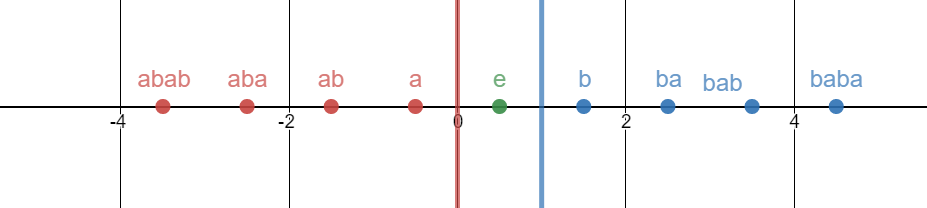
\includegraphics[width=1\textwidth]{images/1-05-d_inf_ab_2.png}
    \caption{The images of $abab[(0.5,0)]$ and $baba[(0.5,0)]$.}
\end{figure}

\end{frame}

\begin{frame}{Properties of this Group}

\begin{proposition}

Let $a$ be the reflection that fixes $x=0$ and $b$ the reflection $x=1$, and let $D_\infty$ be the group
generated by $a$ and $b$. Then every element of $D_\infty$ can be expressed as an alternating product of
$a$'s and $b$'s. Furthermore, if $n\in \mathbb{N}$, then the following hold:

\begin{enumerate}
  \item $abab\ldots abab=(ab)^{n}$ is the horizontal translation described by $(x,y)\rightarrow (x-2n,y)$.
  \item $baba\ldots baba=(ba)^{n}$ is the horizontal translation described by $(x,y)\rightarrow (x+2n,y)$.
  \item $baba\ldots bab=(ba)^{n-1}b$ is the reflection that fixes $x=n$.
  \item $abab\ldots aba=(ab)^{n-1}a$ is the reflection that fixes $x=-n$.
\end{enumerate}

\end{proposition}

\end{frame}

\begin{frame}{Infinite Dihedral Groups}

We prove $(1)$ and $(3)$ and observe how similar the other other cases are after the proof. We will prove
the statement $P(k)$ by induction where $P(k)$ states that $(ab)^{k}=(x-2k,y)$ for a fixed $k$. \\~\\

\pause{}

The base case when $k=0$ is pretty straight forward as $e[(x,y)]=(ab)^{0}[(x,y)]=(x,y)=(x-2(0),y)$. \\~\\

\pause{}

We assume the inductive hypothesis and attempt to prove this holds when $k=n+1$. We see that
$(ab)^{n+1}[(x,y)]=(ab)(ab)^{n}[(x,y)]$. Applying the inductive hypothesis gives us that
$(ab)(ab)^{n}[(x,y)]=ab[(x-2n,y)]$. Applying $b$ gives us $ab[(x-2n,y)]=a[(2-(x-2n),y)]$. Applying $a$
gives us $(x-2(n+1),y)$. So $P(n+1)$ holds.

\end{frame}

\begin{frame}{Infinite Dihedral Groups}

To prove $(3)$, we simply look at it algebraically. We note that:

\begin{align*}
(ba)^{n-1}b[(x,y)]
&= (ba)^{n-1}[(2-x,y)] \\
&= ((2-x)+2(n-1),y) \\
&= (2n-x,y)
\end{align*}

We see that $(ba)^{n-1}b[(n,y)]=(n,y)$. This completes the proof of (3) and (4) is identical to this.
\end{frame}

\begin{frame}{Infinite Dihedral Groups}

We can conclude that if translations $w_{1}=(ab)^{n}$ and $w_{2}=(ba)^{n}$ and reflections
$w_{3}=(ba)^{n-1}b$, and $w_{4}=(ab)^{n-1}a$, then for $i\neq j$:

\begin{itemize}
  \item $\Rightarrow w_{i}\neq w_{j}$, and
  \item $w_{i}[(x,y)]\neq w_{j}[(x,y)]$.
\end{itemize}

\end{frame}

\begin{frame}{Tiling of the Plane}

We see that the axes of reflections help us create a tiling of the plane. This can be seen by 
``rolling'' a piece of paper that has one edge painted red and the other blue.

\begin{figure}[h]
    \centering
    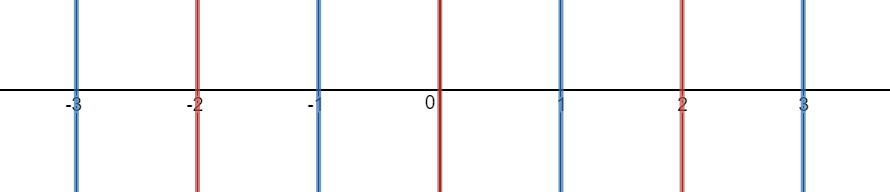
\includegraphics[width=1\textwidth]{images/2-02-Tiling.png}
    \caption{The tiling of the plane caused by $a,b\in D_\infty$.}
\end{figure}

\end{frame}

\begin{frame}{The ``Two Wrongs make a Right'' Property}

The tiling property is not only for decoration. It allows us to compute $w=w_{1}w_{2}\ldots w_{n}$, s.t.
$w_{i}\in {a,b}$ in a different and interesting way. We first see this by example. We can evaluate
$baba[(0,5,0)]$ below ``the right way''.

\begin{figure}[h]
    \centering
    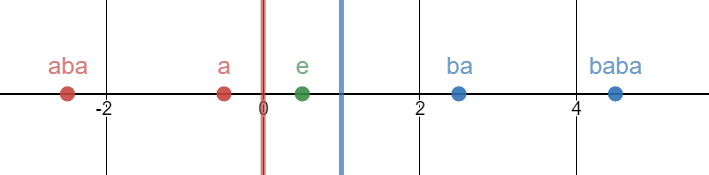
\includegraphics[width=1\textwidth]{images/2-03-Computing_baba.png}
    \caption{Computing $baba$ the correct way.}
\end{figure}

\end{frame}

\begin{frame}{The ``Two Wrongs make a Right'' Property}

Now we do it again while making two mistakes below:

\begin{figure}[h]
    \centering
    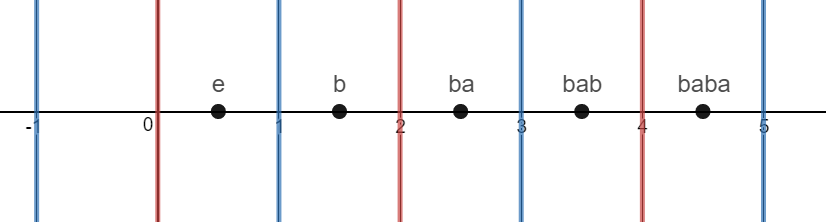
\includegraphics[width=1\textwidth]{images/2-04-Wrong_Way.png}
    \caption{Computing $baba$ when making 2 mistakes.}
\end{figure}

\end{frame}

\begin{frame}{Cayley Graph of $D_\infty$}

Furthermore, we can create our Cayley graph with the following steps:  

\begin{enumerate}
  \item Start with a vertex labelled $\varepsilon$
  \item Draw a vertex to the left and right of the vertex labelled $\varepsilon$ and label them $a$ and
  $b$, respectively, while labelling the edges $a$ and $b$, respectively.
  \item Draw a vertex to the left of the vertex labelled $a$ and right of the vertex labelled $b$ and label
  them $ba$ and $ab$, respectively, while labelling the edges $b$ and $a$, respectively.
  \item Repeat forever.
\end{enumerate}

\end{frame}

\begin{frame}{Cayley Graph of $D_\infty$}

It looks like so:

\begin{figure}[h]
    \centering
    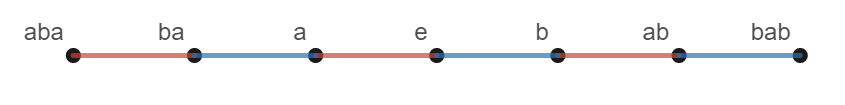
\includegraphics[width=1\textwidth]{images/2-01-Cayley_Graph.png}
    \caption{The Cayley graph of $D_\infty$.}
\end{figure}

\end{frame}

\begin{frame}{The Fundamental Domain of $D_\infty$}

Note that a single vertex and its two half edges are all that are needed for the fundamental domain.
\begin{figure}[h]
    \centering
    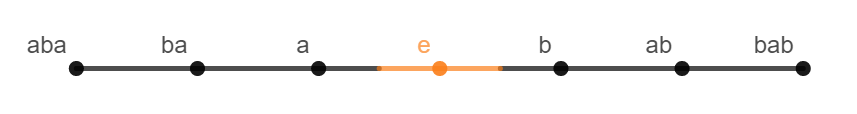
\includegraphics[width=1\textwidth]{images/2-01-01-Fundamental_Domain.png}
    \caption{The Fundamental Domain of $D_\infty$.}
\end{figure}

\end{frame}

\begin{frame}{Generating a Strict Subgroup $D_\infty$ Isomorphic to $D_\infty$}

We note that $D_\infty$ exhibits some interesting behaviour.

\begin{proposition}

The subgroup $H$ of $D_\infty$ generated by $\{a,bab\}$ is a subgroup of index 2 that is isomorphic to
$D_\infty$.

\end{proposition}

We need to show this in steps:

\begin{enumerate}
  \item Define a map $\varphi:H\rightarrow D_{\infty}$. 
  \item Show $\varphi$ is well-defined and a group homomorphism.
  \item Show $\varphi$ is surjective.
  \item Show $\ker(\varphi)={1}$
  \item Show $H$ has index 2.
\end{enumerate}

\end{frame}

\begin{frame}{Generating a Strict Subgroup $D_\infty$ Isomorphic to $D_\infty$}

\textbf{Step 1}: Let's let $\alpha=a$ and $\beta=bab$. Now, define $\varphi$ to be such that
$\varphi(\alpha)=a$, $\varphi(\beta)=b$, and for an arbitrary element $\varphi(x_{1}x_{2}\ldots
x_{n})=\varphi(x_{1})\varphi(x_{2})\ldots \varphi(x_{n})$ where $x_{i}\in {\alpha, \beta}$. \\~\\

\pause{}

\textbf{Step 2}: To see that this map is well-defined, we first recall from the previous proposition that
elements of $D_\infty$ are uniquely described by $a$'s and $b$'s. So it's very clear that $\forall$ words
$w,w'\in H, w=w' \Rightarrow \varphi(w)=\varphi(w')$. 

\pause{}

We note that $\varphi$ must be a homomorphism simply from its definition.

\end{frame}

\begin{frame}{Generating a Strict Subgroup $D_\infty$ Isomorphic to $D_\infty$}

\textbf{Step 3}: We want to show $\varphi$ is surjective. However, by our definition of $\varphi$, every
generator ${a,b}$ of $D_\infty$ has some word in $H$ mapping to it. Therefore, $\varphi$ is surjective.
\\~\\

\pause{}

\textbf{Step 4}: We want to show that $\ker(\varphi)={1}$. We first note that $\varphi(\alpha)\neq 1$ and
$\varphi(\beta)\neq 1$.  

\pause{}

So assume $x\in H$ such that $x=x_{1}x_{2}\ldots x_{n}$. First, assume $n\geq 1$ is even and starts with
$\alpha$. Then $x=(\alpha\beta)^{n/2}$ and so $\varphi(x)=(ab)^{n/2}\neq 1_{D_\infty}$ by the first
proposition. 

\pause{}

Similarly, we see what happens when $n$ is odd. So $\ker(\varphi)={1}$.

\end{frame}

\begin{frame}{Generating a Strict Subgroup $D_\infty$ Isomorphic to $D_\infty$}

We conclude that $H$ and $D_\infty$ are isomorphic to each other. \\~\\

\pause{}

\textbf{Step 5}: We want to show that the index of $H$ is 2. We show this by proving $D_\infty=H\cup bH$.
\pause{} To see this, note that $H=\{ w | w $ has an even amount of $b$'s $\}$. Left multiplying every
element of $H$ by $b$ gives us the remaining elements of $D_\infty$ with no overlap. So $H$ has index 2 in
$D_\infty$.

\end{frame}

\begin{frame}{What comes next}

We've looked at $D_\infty$ and how it's generated by 2 reflections. Next, we'd like to see a group that is
generated by 3 reflections and any interesting different or similar properties that arise.

\end{frame}

%%%%%%%%%%%%%%%%%%%%%%%%%%%%%%%%%%%%%%%%%%%%%%%%%%%%%%%%
%%%%%% GROUPS GENERATED BY THREE REFLECTIONS BEGIN %%%%%
%%%%%%%%%%%%%%%%%%%%%%%%%%%%%%%%%%%%%%%%%%%%%%%%%%%%%%%%

\section{Groups Generated by Three Reflections}

\begin{frame}{Groups Generated by 3 Reflections}

There are many groups that are generated by three reflections. These were studied by Jacques Tits who called them \textit{Coxeter Groups}. 

For simplicity, we'll primarily focus on $W_{333}$. 

\end{frame}

\begin{frame}{Orbit of $e$ in $W_{333}$}

Suppose we defined three reflections on the Cartesian plane:

\begin{itemize}
  \item \textcolor{red}{$r[(x,y)]=(x,-y)$}
  \item \textcolor{blue}{$b[(x,y)]=(\frac{3-x-\sqrt{3}y}{2},\frac{3-\sqrt{3}x+y}{2})$}
  \item \textcolor{green}{$g[(x,y)]=(\frac{-3-x+\sqrt{3}y}{2},\frac{3+\sqrt{3}x+y}{2})$}
\end{itemize}

Choose \textcolor{orange}{$e$} to be the barycenter/centroid. What's its orbit?

\end{frame}

\begin{frame}{Orbit of $e$ in $W_{333}$}

\begin{figure}[h]
    \centering
    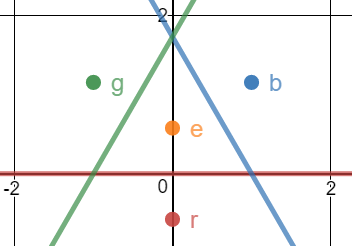
\includegraphics[width=0.7\textwidth]{images/6-01-rbg-rbg-1.png}
    \caption{The axes of reflections \textcolor{red}{$r$}, \textcolor{blue}{$b$}, \textcolor{green}{g} and the points \textcolor{red}{$r$}, \textcolor{blue}{$b$}, \textcolor{green}{g}.}
\end{figure}

\end{frame}

\begin{frame}{Orbit of $e$ in $W_{333}$}

\begin{figure}[h]
    \centering
    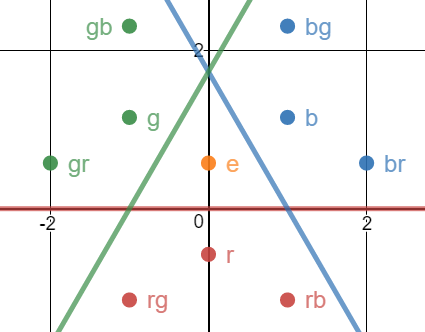
\includegraphics[width=.65\textwidth]{images/6-02-rbg_rbg_2.png}
    \caption{The points \textcolor{red}{$r$}, \textcolor{blue}{$b$}, \textcolor{green}{g}, \textcolor{red}{$rb$}, \textcolor{red}{$rg$}, \textcolor{blue}{$br$}, \textcolor{blue}{$bg$}, \textcolor{green}{gr}, \textcolor{green}{gb}.}
\end{figure}

\end{frame}

\begin{frame}{Orbit of $e$ in $W_{333}$}

\begin{figure}[h]
    \centering
    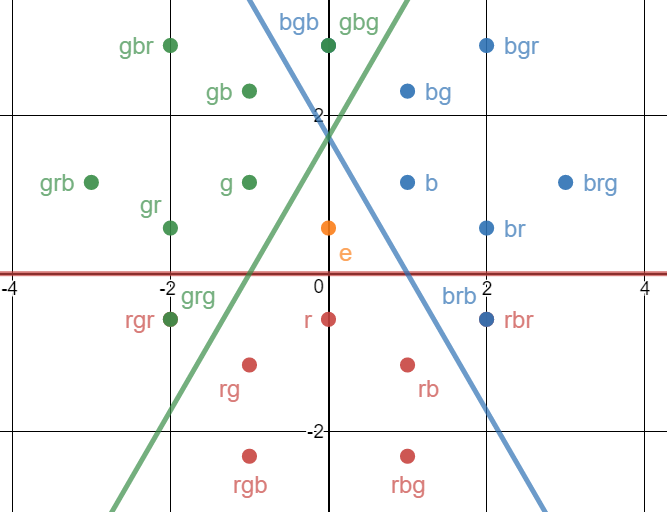
\includegraphics[width=.65\textwidth]{images/6-03-rbg_rbg_3.png}
    \caption{The points consisting of 0, 1, 2, and 3 reflections.}
\end{figure}

\end{frame}

\begin{frame}{Tiling of the plane under $W_{333}$}

How does the tiling look? 

\pause{}

\begin{figure}[h]
    \centering
    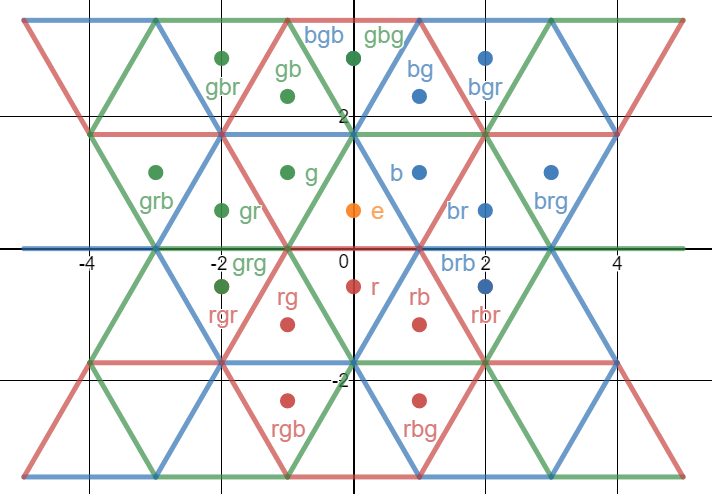
\includegraphics[width=.65\textwidth]{images/6-05-rbg_rbg_3-tiling.png}
    \caption{The tiling of the group.}
\end{figure}

\end{frame}

\begin{frame}{Cayley Graph of $W_{3,3,3}$}

Suppose our generating set is $S=\{r,b,g\}$. What's $\Gamma_{W_{3,3,3},S}$

\pause{}

\begin{itemize}
\item $W_{3,3,3}$ acts transitively on the barycenters of each triangle
\item This gives us the orbit of $x$ under $W_{3,3,3}$
\end{itemize}
\end{frame}

\begin{frame}{Cayley Graph of $W_{3,3,3}$}
\begin{figure}[h]
    \centering
    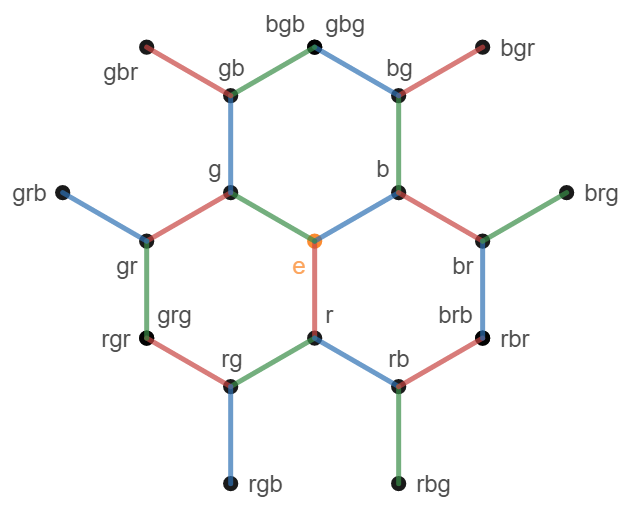
\includegraphics[width=.6\textwidth]{images/6-06-rbg_rbg_3-cayley.png}
    \caption{The Cayley graph of the group looking like a hexagonal tiling.}
\end{figure}

\end{frame}

\begin{frame}{Fundamental Domain of $W_{333}$}

We recall Theorem 1.55 that states $S=\{g\in G | g \ne e$ and $gF \cap F\}$ for a generating set $S$.

\pause{}

\begin{figure}[h]
    \centering
    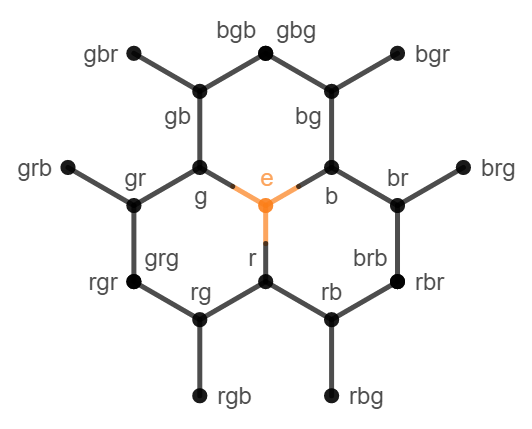
\includegraphics[width=.5\textwidth]{images/6-07-rbg_rbg_3-fundamental_domain.png}
    \caption{The Fundamental Domain}
\end{figure}

\end{frame}

\begin{frame}{Other Groups Generated by Three Reflections}

\begin{itemize}
  \item $W_{2,4,4}$, the group generated by triangles with interior angles $\{\pi/2,\pi/4,\pi/4\}$
  \item $W_{2,3,6}$, the group generated by triangles with interior angles $\{\pi/2,\pi/3,\pi/6\}$
  \item Similar, but they have their ``quirks''
\end{itemize}

\end{frame}

\begin{frame}{Question 7}

Draw the Cayley Graphs of $W_{2,4,4}$ and $W_{2,3,6}$.

\end{frame}

\begin{frame}{$W_{2,4,4}$}

\begin{figure}[h]
    \centering
    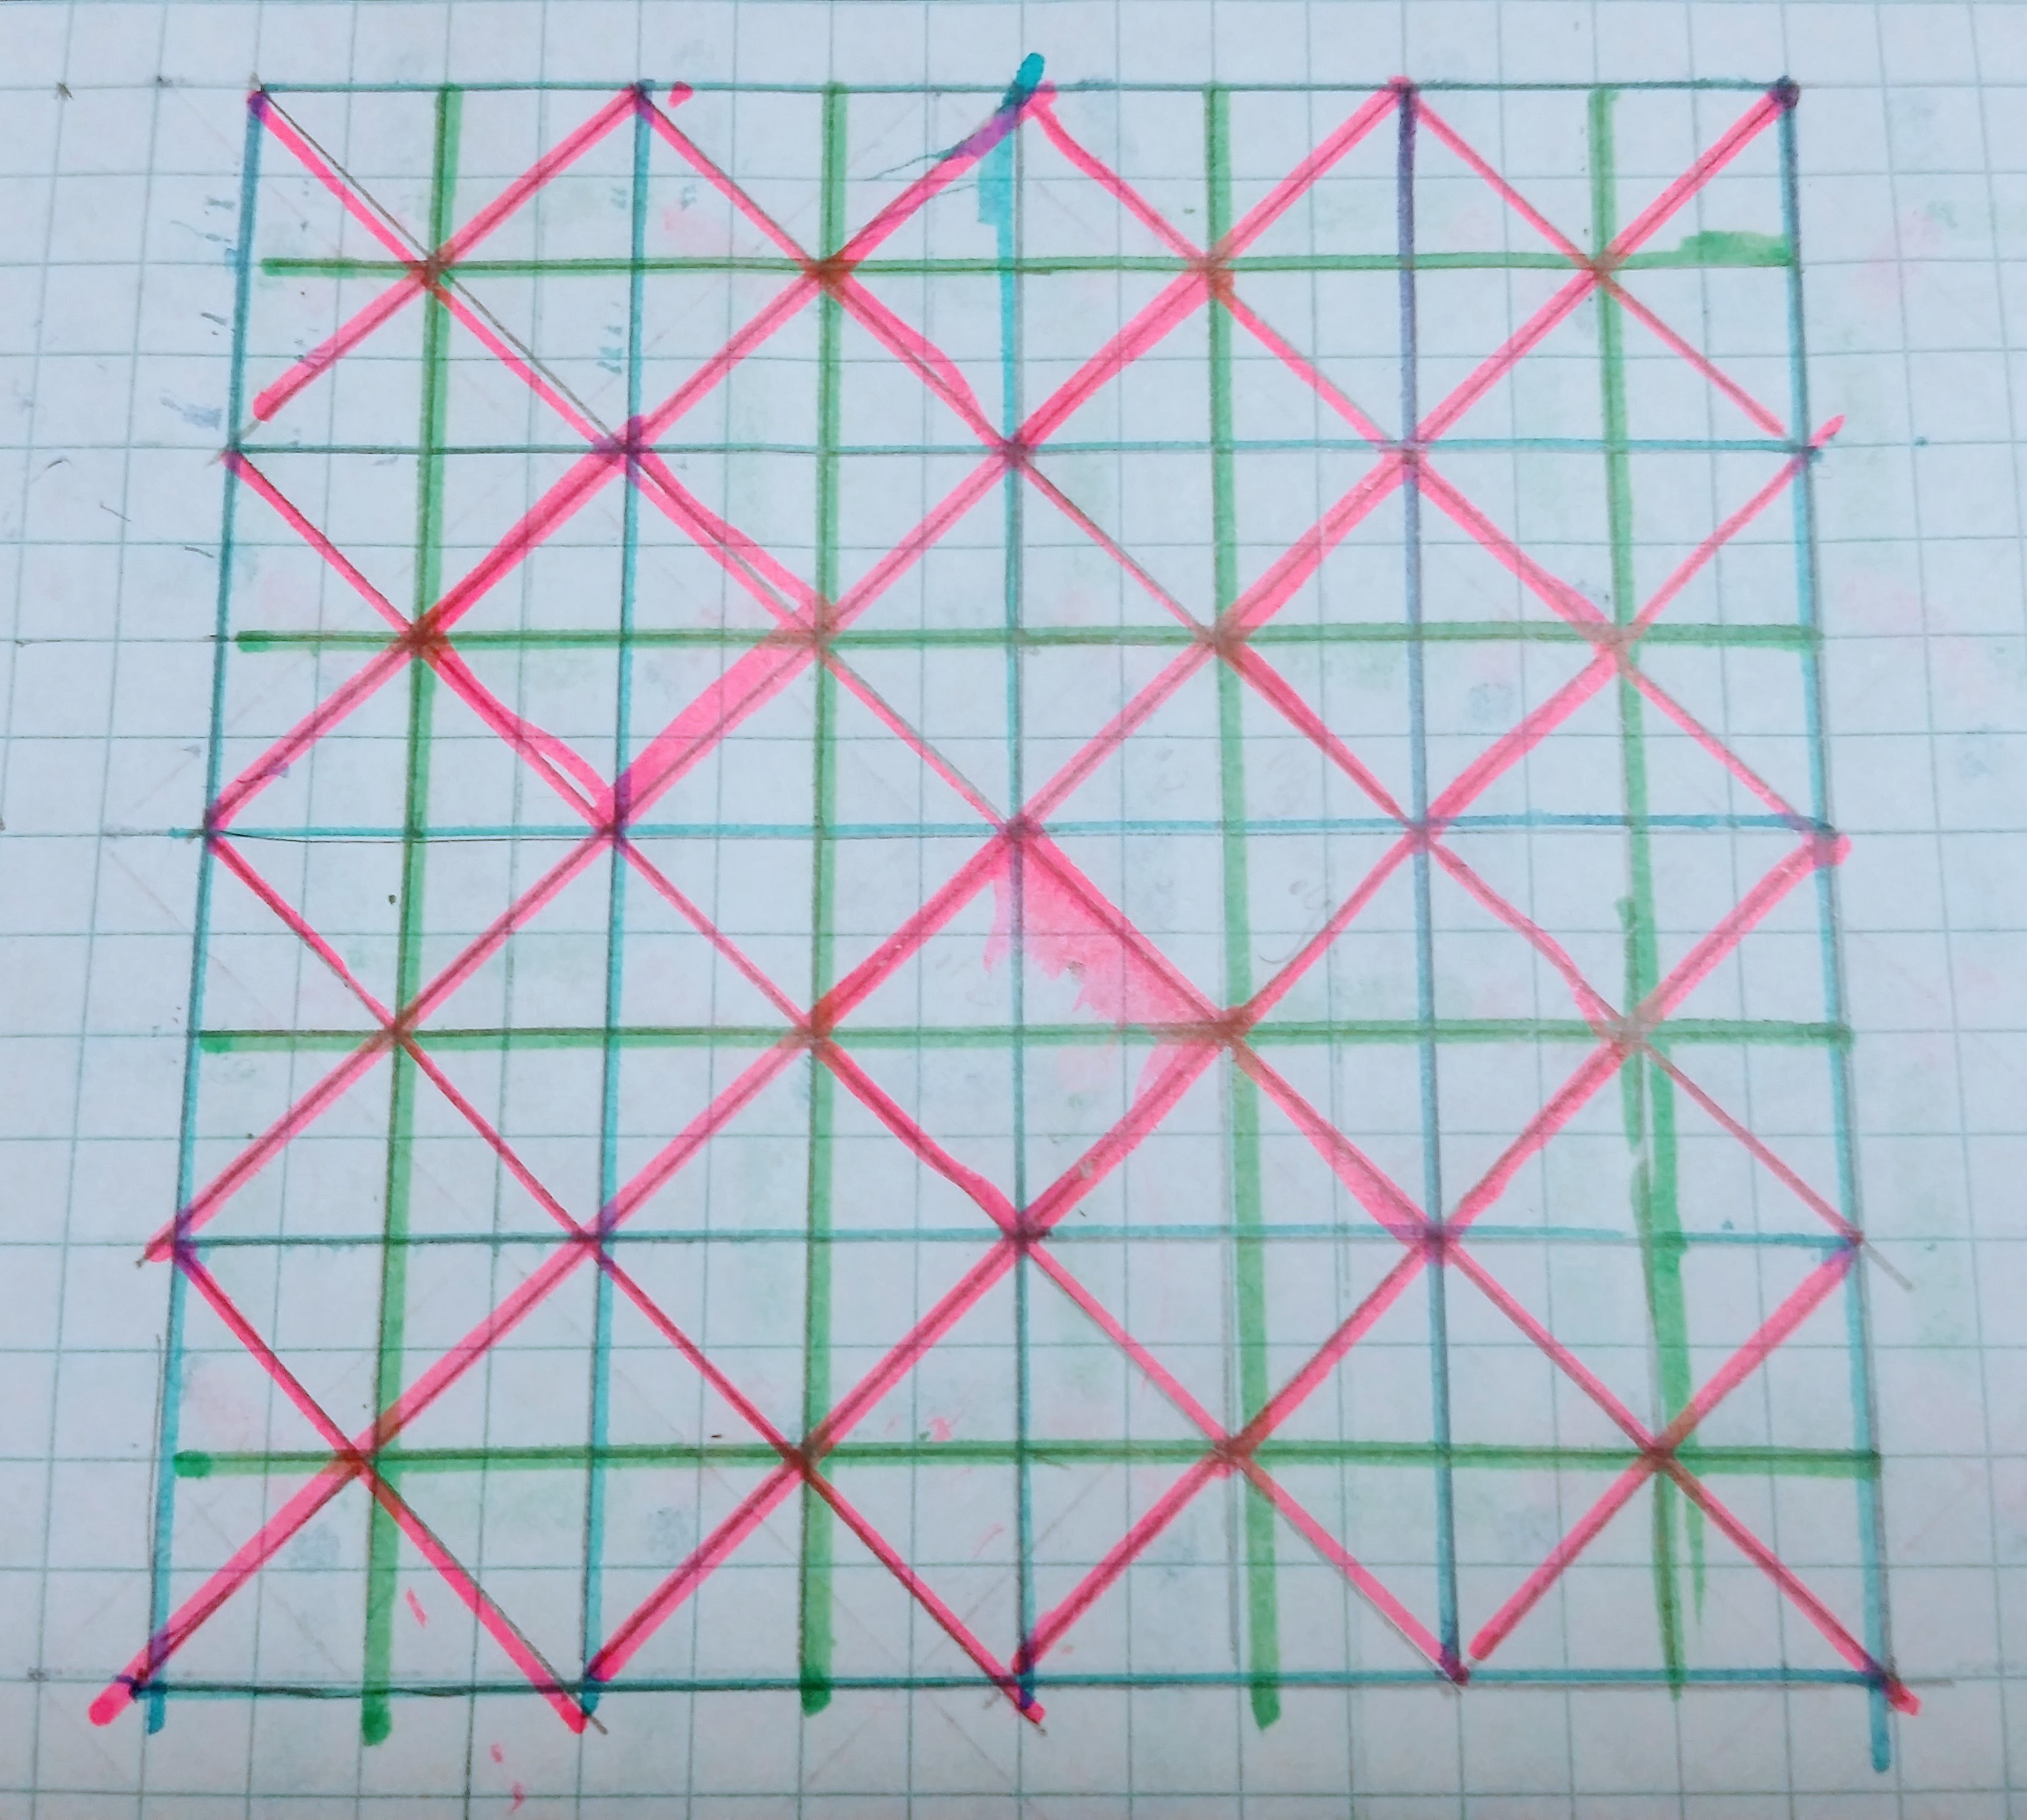
\includegraphics[width=.5\textwidth]{images/7-03-W_244_tiling.png}
    \caption{The tiling generated by triangles with interior angles $\frac{\pi}{2},\frac{\pi}{4},\frac{\pi}{4}$}
\end{figure}

\end{frame}

\begin{frame}{$W_{2,4,4}$}

\begin{figure}[h]
    \centering
    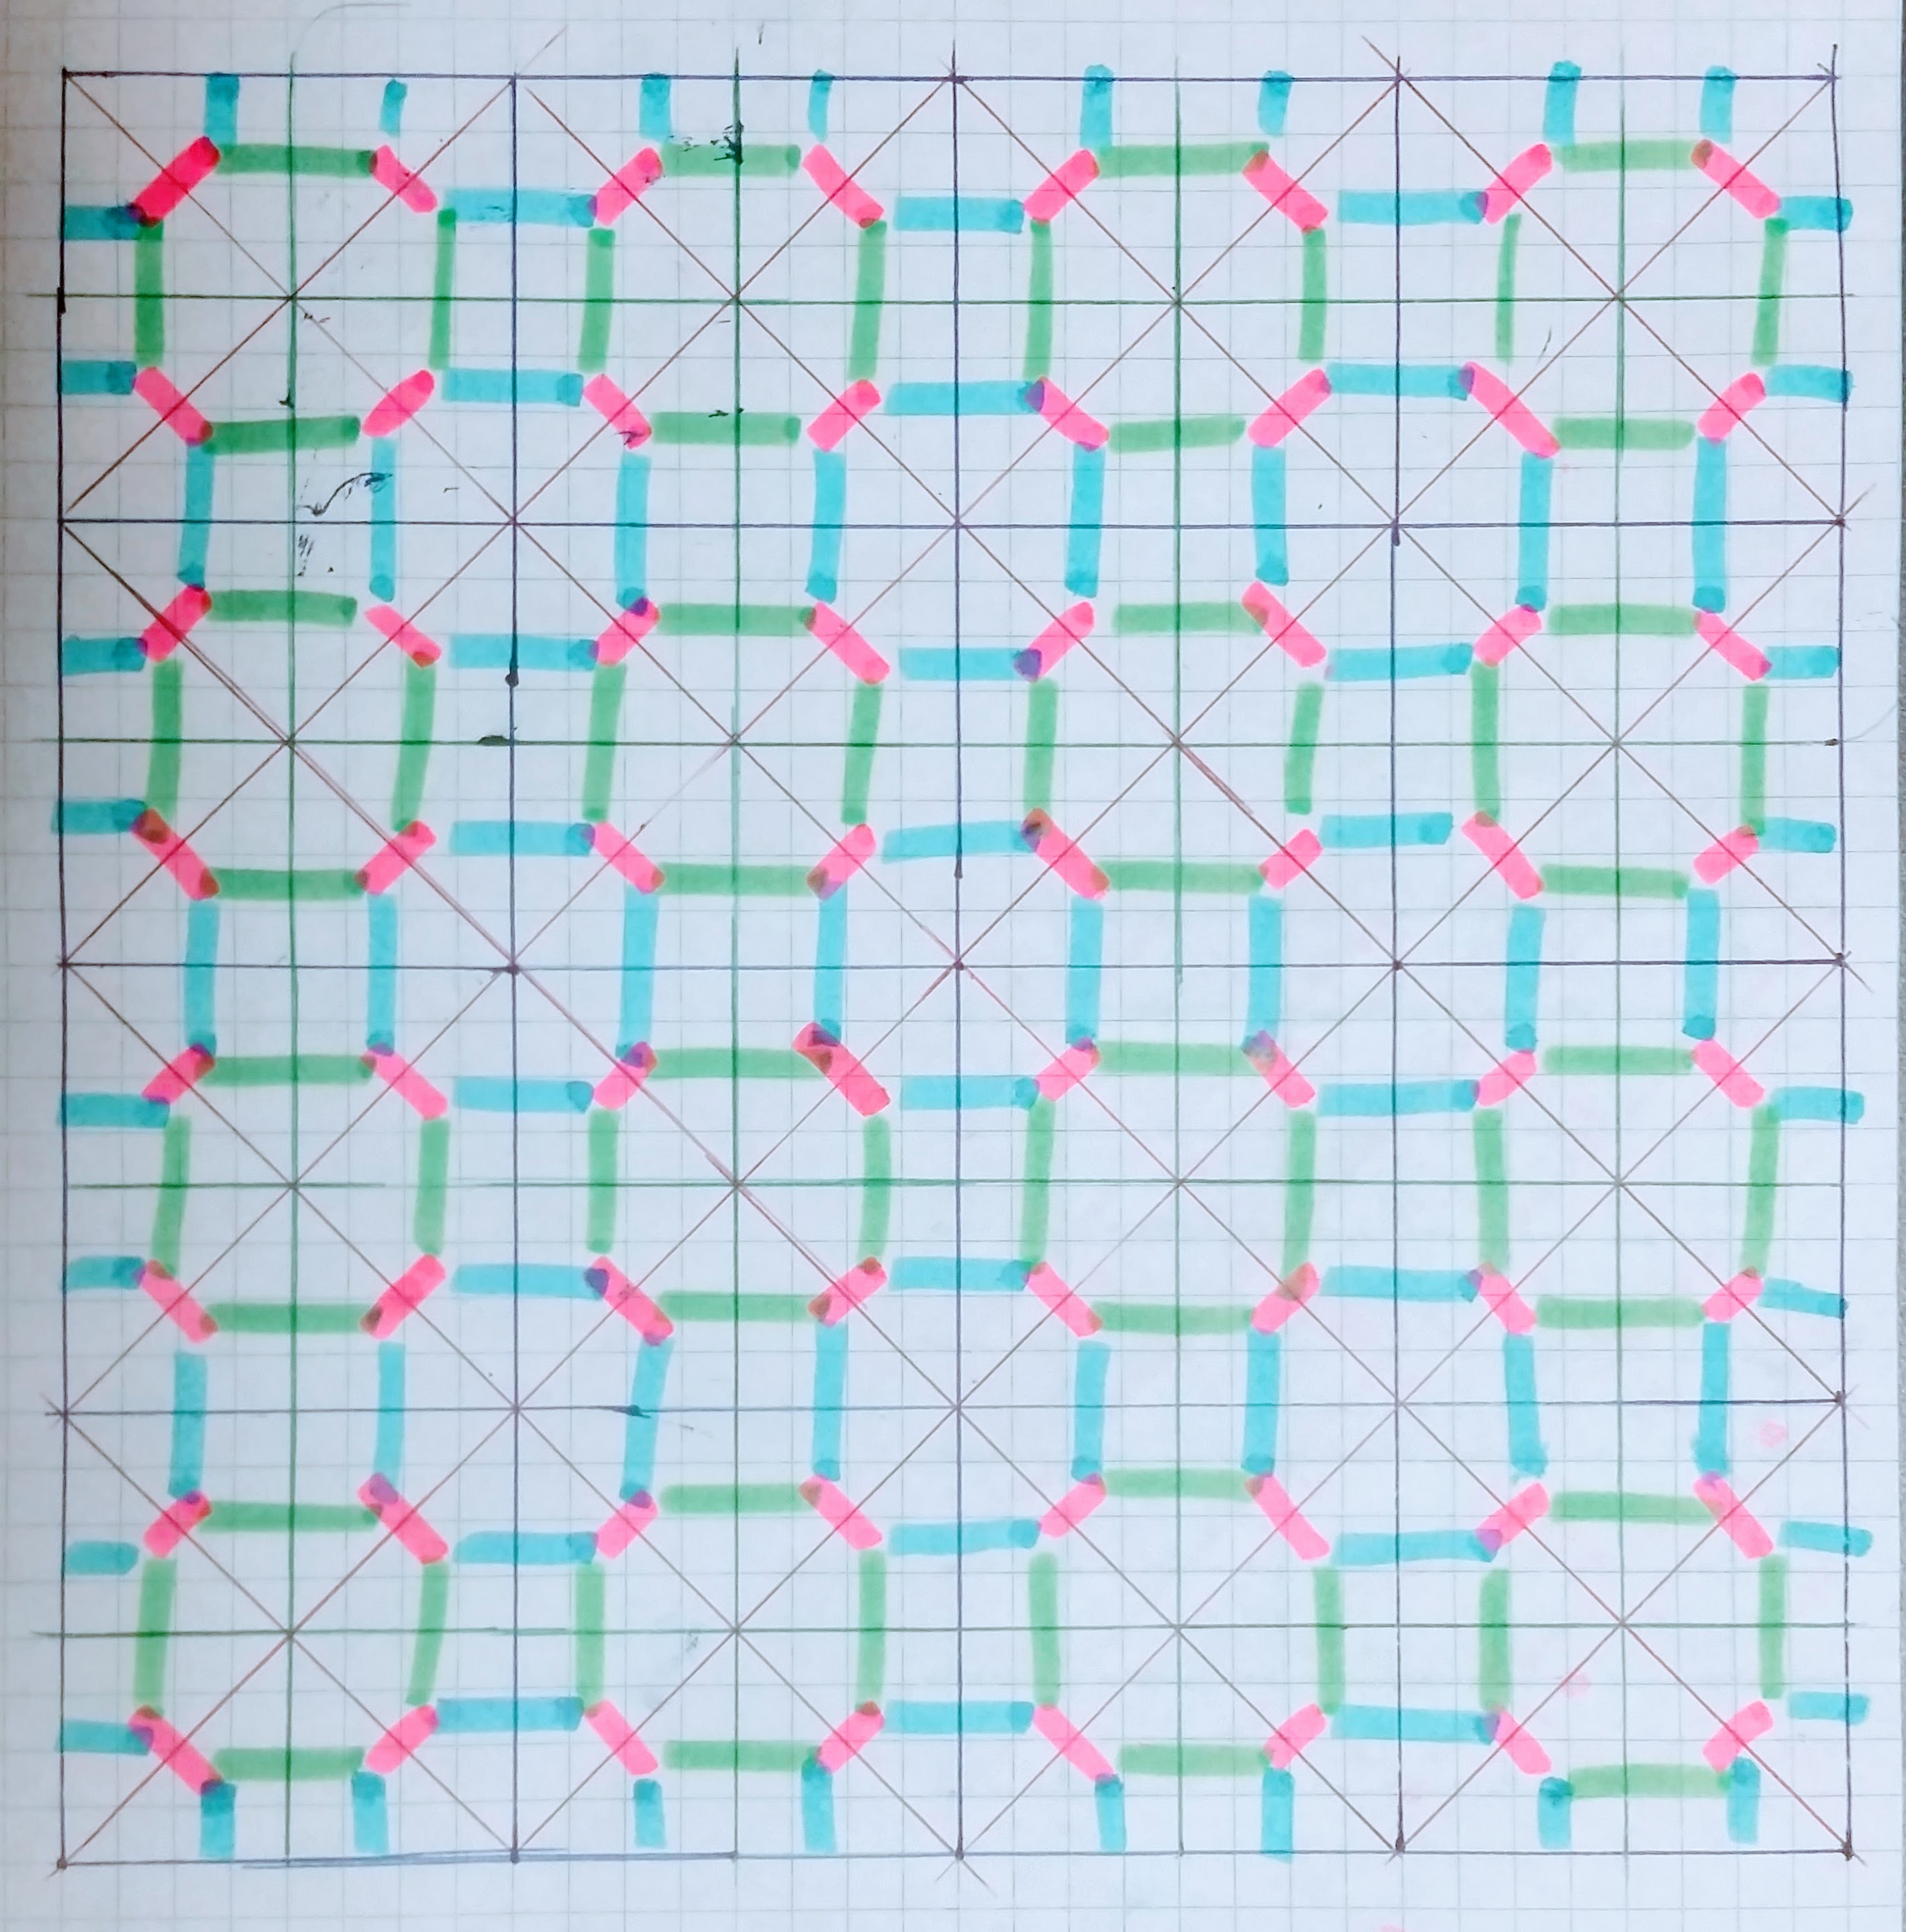
\includegraphics[width=.5\textwidth]{images/7-04-W_244_cayley_graph.png}
    \caption{The Cayley graph of the group $W_{2,4,4}$.}
\end{figure}

\end{frame}

\begin{frame}{$W_{2,3,6}$}

\begin{figure}[h]
    \centering
    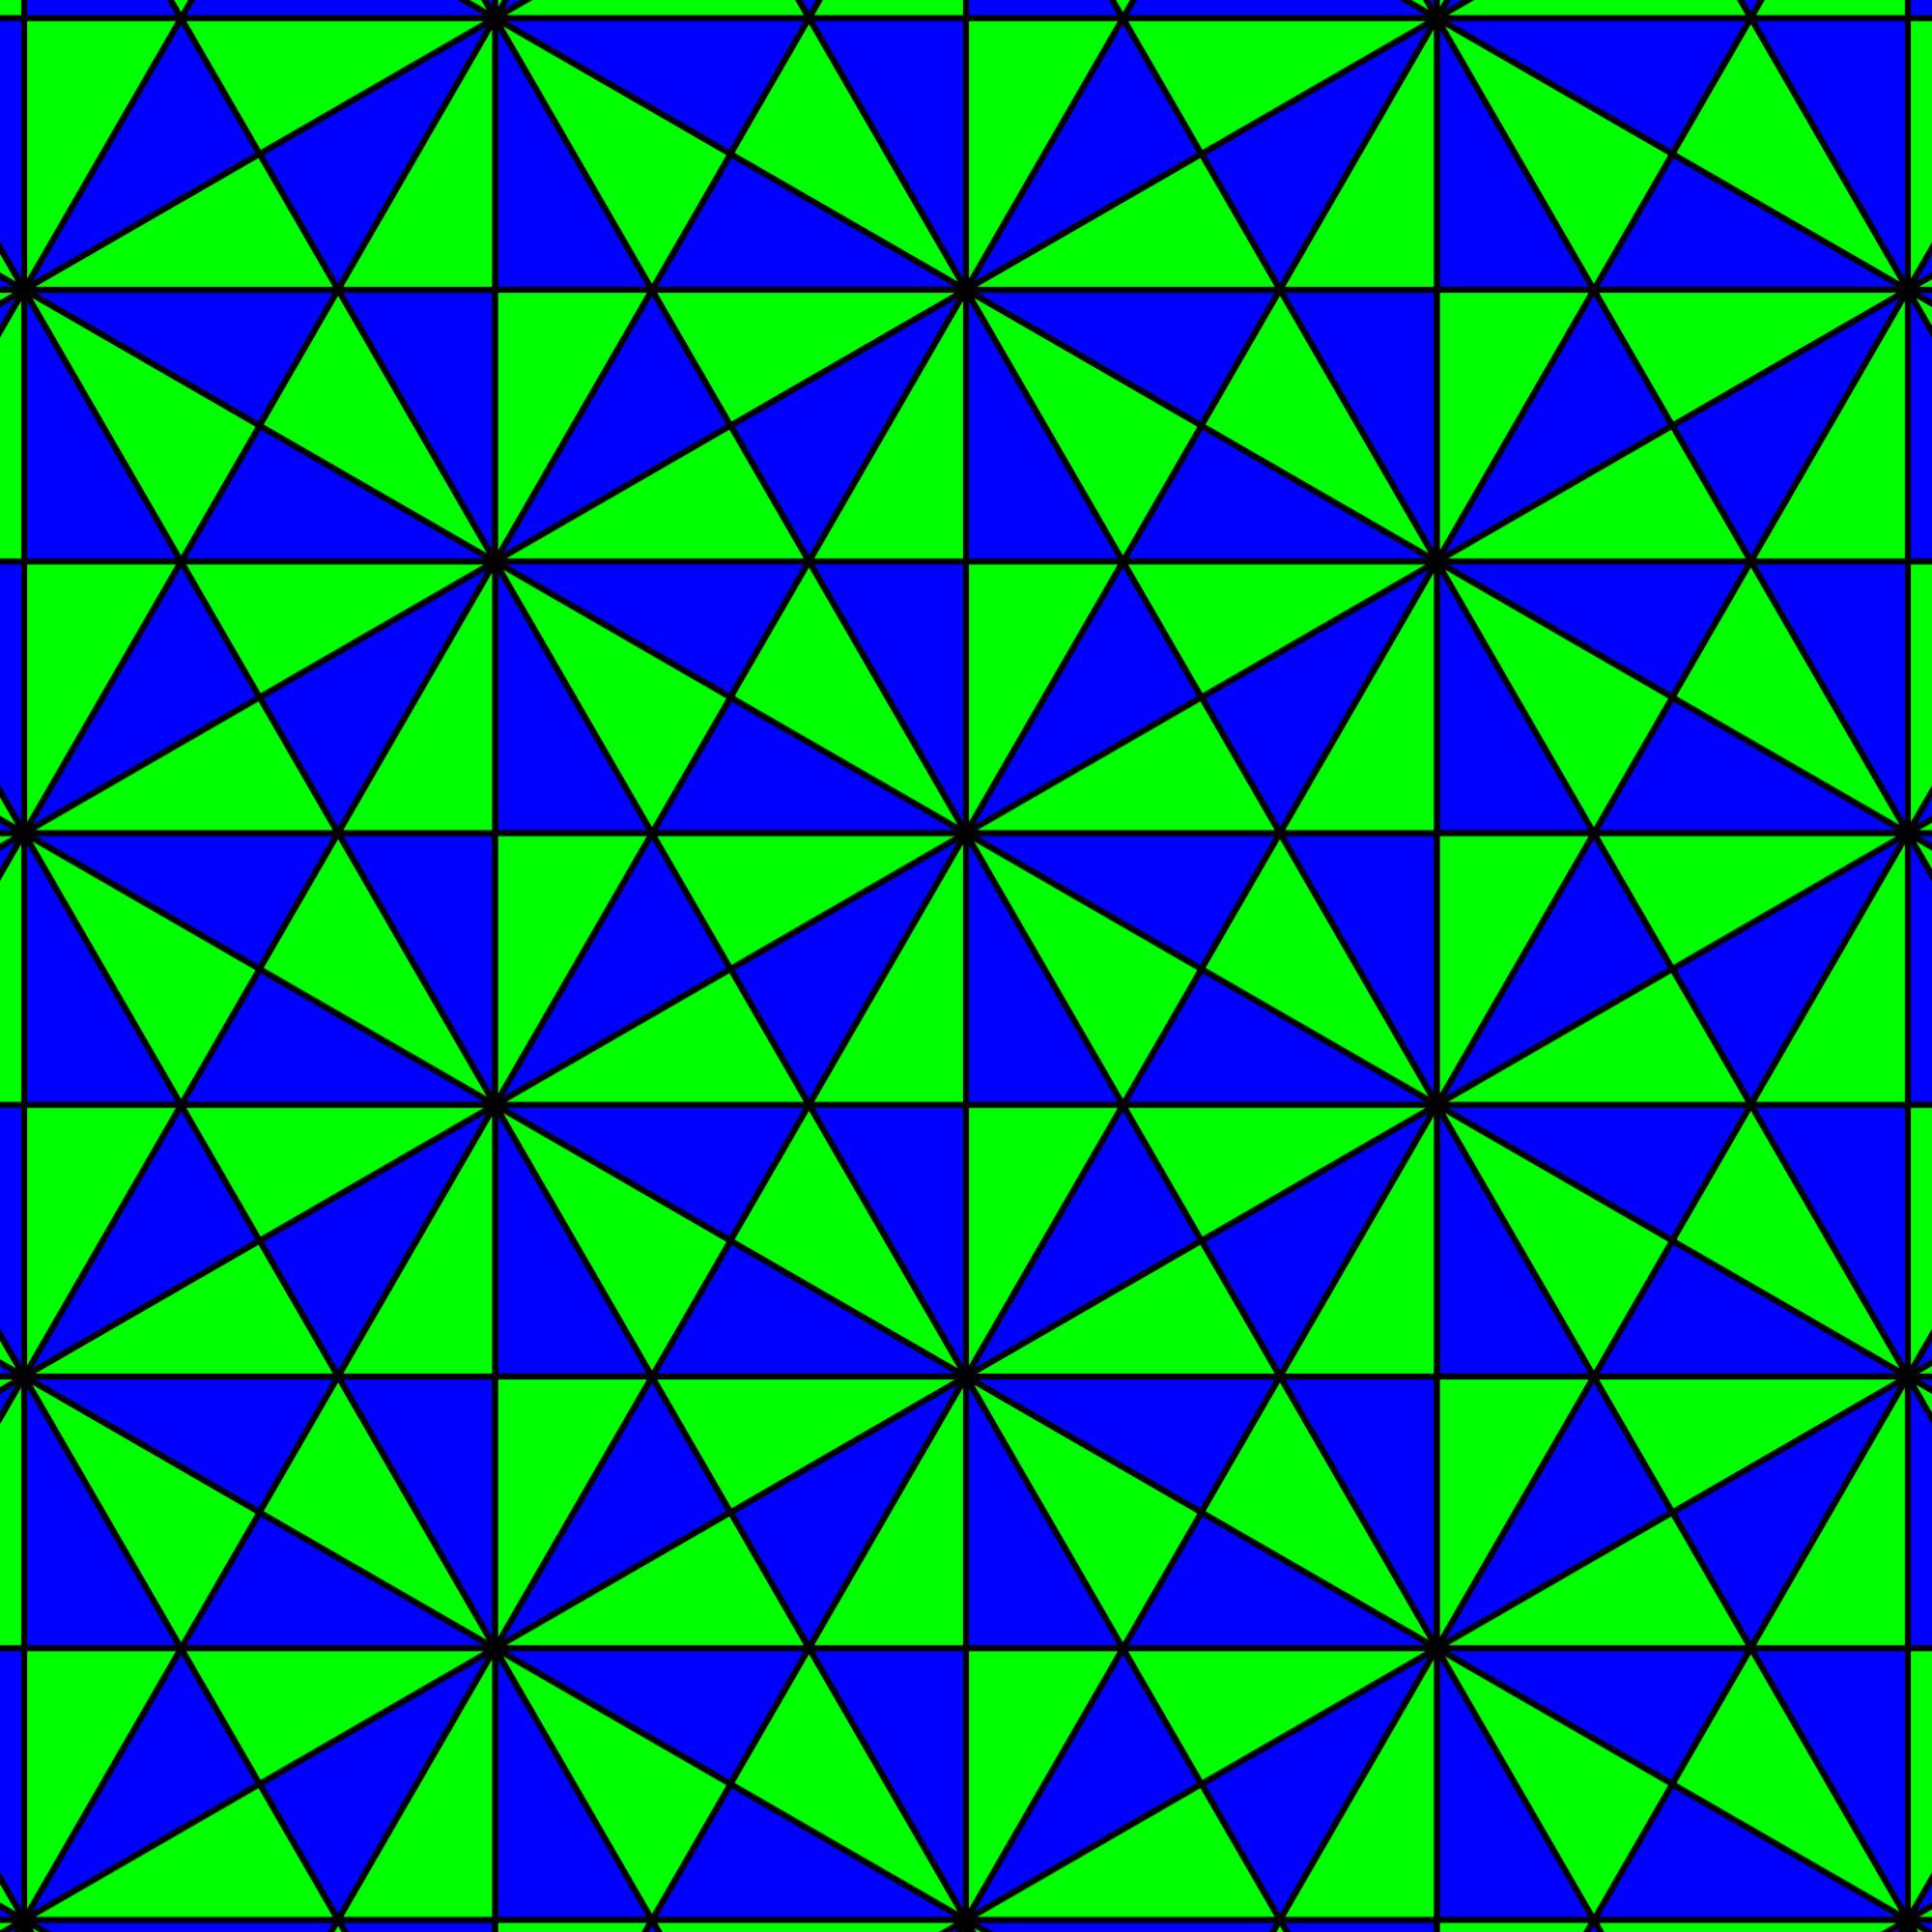
\includegraphics[width=.5\textwidth]{images/7-02-W_236_cayley_graph.png}
    \caption{The tiling generated by triangles with interior angles $\frac{\pi}{2},\frac{\pi}{3},\frac{\pi}{6}$}
\end{figure}

\end{frame}

\begin{frame}{$W_{2,3,6}$}

\begin{figure}[h]
    \centering
    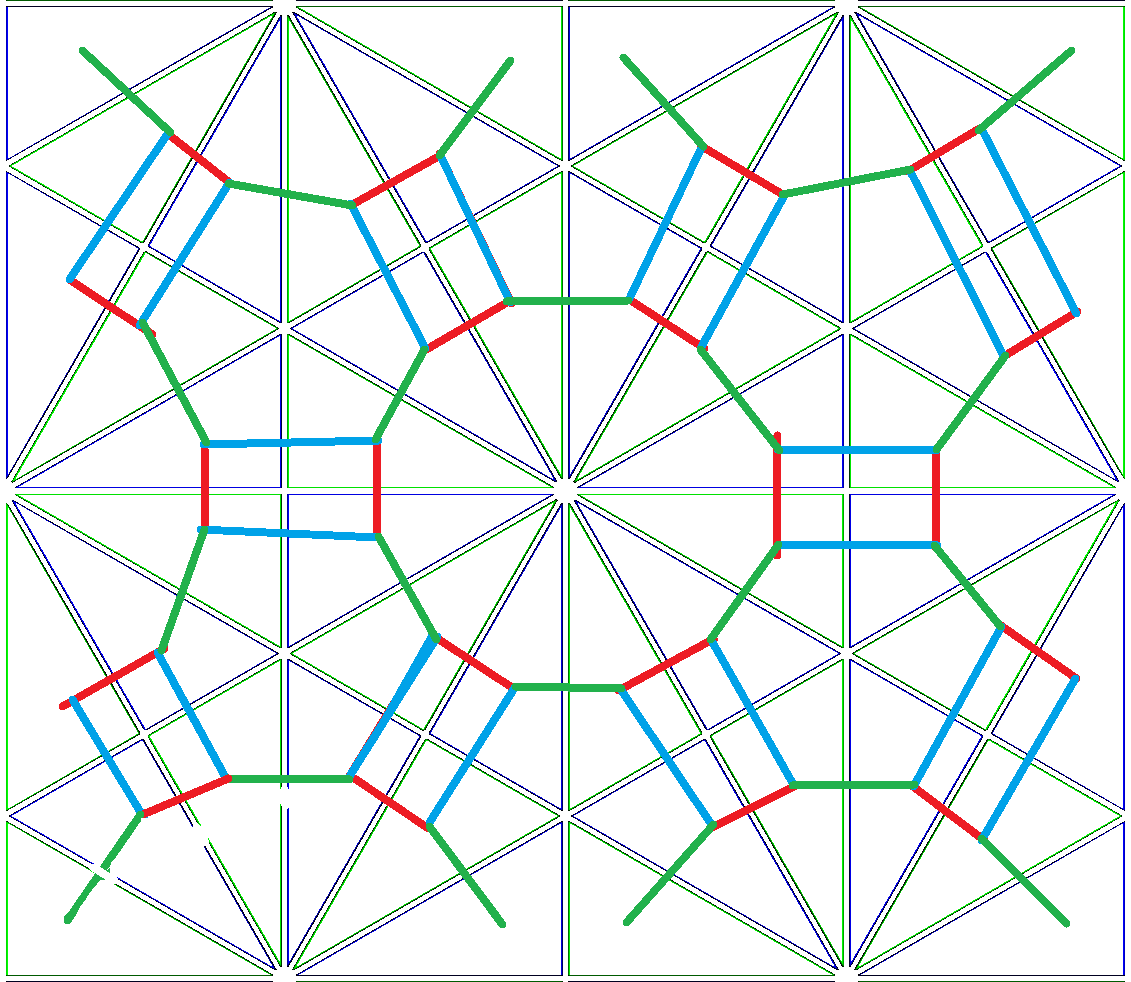
\includegraphics[width=.55\textwidth]{images/7-01-W_236_tiling.png}
    \caption{The Cayley graph of the group $W_{2,3,6}$.}
\end{figure}

\end{frame}

\section{Extra Questions}

\begin{frame}{Question 5}

Tile the plane with squares. Let $W$ represent the group generated by the 4 reflections of each side of a
square. Prove that $W\cong D_{\infty} \oplus D_{\infty}$.

Suppose we defined three reflections on the Cartesian plane:

\begin{itemize}
  \item \textcolor{red}{$r[(x,y)]=(-x,y)$}
  \item \textcolor{blue}{$r[(x,y)]=(2-x,y)$}
  \item \textcolor{Fuchsia}{$r[(x,y)]=(x,-y)$}
  \item \textcolor{green}{$r[(x,y)]=(x,2-y)$}
\end{itemize}

Choose \textcolor{orange}{$e$} to be the barycenter/centroid. What's its orbit?

\end{frame}

\begin{frame}{Question 5}

\begin{figure}[h]
    \centering
    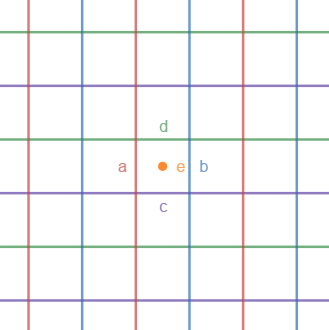
\includegraphics[width=.5\textwidth]{images/8-01-Tiling_of_D_infty_D_infty.png}
    \caption{The tiling of the group $W$.}
\end{figure}

\end{frame}

\begin{frame}{Question 5}

Firstly, let's look at an arbitrary point in the tiling, say $w=bcadcabad$. \pause{} We note that vertical
and horizontal actions can be interchanged. That is $\{a,b\}$ commute with $\{c,d\}$. \pause{} So this word
can be rewritten as $w=baabacdcd=w_{h}w_{v}$  where $w_h,w_v$ represent the sequence of horizontal and vertical
actions, respectively. \pause{} Each of these are words in their own instances of $D_\infty$.

\end{frame}

\begin{frame}{Question 5}

More formally, let $D_\infty=<a,b|a^2,b^2>$ and let $\phi:W\rightarrow D_\infty \oplus D_\infty$ such that:

 \pause{}

\begin{itemize}
  \item $\phi(a)=(a,e)$
  \item $\phi(b)=(b,e)$
  \item $\phi(c)=(e,a)$
  \item $\phi(d)=(e,b)$
\end{itemize}

\end{frame}

\begin{frame}{Question 5}

What's left to do here is to show that:

\begin{itemize}
\item $\phi$ is onto
\item $\ker(\phi)$ is trivial
\item Show that this is a valid homomorphism
\end{itemize}

Let $x_1,x_2, \ldots x_n \in W$ and  $y_1,y_2, \ldots y_j\in \{a,b\}$ $z_1,z_2, \ldots z_k\in \{c,d\}$.
Then we can see that:
\begin{align*}
\phi(x_1x_2 \ldots x_n)
&=\phi(y_1y_2 \ldots y_{j}z_{1}z_{2} \ldots z_k)\\
&=\phi(y_1y_2 \ldots y_j)\phi(z_1z_2 \ldots z_k)\\
&=\phi(y_1)\phi(y_2) \ldots \phi(y_j)\phi(z_1)\phi(z_2) \ldots \phi(z_k)\\
&=\phi(x_1)\phi(x_2) \ldots \phi(x_n)
\end{align*}
\end{frame}

\begin{frame}{Question 6}

Prove that $\Z \oplus \Z$ is a subgroup of $W_{3,3,3}$.\\

\pause{}

Let $V=\{w={a_1a_2\ldots a_n} | a_i\in\{(bgr)^2,(bgr)^{-2},brbg,(brbg)^{-1}\}\}$, including the empty word.
Here, $(bgr)^2$ denotes a shift in a horizontal direction and $brbg$ denotes a shift in the vertical
direction. Firstly, we see this is a subgroup of $W_{3,3,3}$.

\end{frame}

\begin{frame}{Tiling of the plane under $W_{333}$}

\begin{figure}[h]
    \centering
    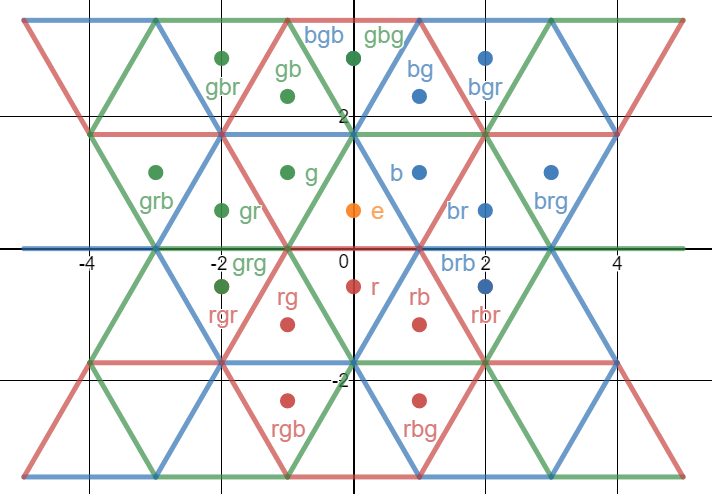
\includegraphics[width=.7\textwidth]{images/6-05-rbg_rbg_3-tiling.png}
    \caption{The tiling of the group.}
\end{figure}

\end{frame}

\begin{frame}{Question 6}

Prove that $\Z \oplus \Z$ is a subgroup of $W_{3,3,3}$.\\

Let $V=\{w={a_1a_2\ldots a_n} | a_i\in\{(bgr)^2,(bgr)^{-2},brbg,(brbg)^{-1}\}\}$, including the empty
word. Here, $(bgr)^2$ denotes a shift in a horizontal direction and $brbg$ denotes a shift in the vertical
direction. Firstly, we see this is a subgroup of $W_{3,3,3}$. Secondly, we see that a mapping
$\phi:V\rightarrow \Z \oplus \Z$ such that $\phi((bgr)^2)=(1,0)$, $\phi((bgr)^{-2})=(-1,0)$,
$\phi(brbg)=(0,1)$, $\phi((brbg)^{-1})=(0,-1)$. 


\end{frame}

\begin{frame}{Question 6}

We need to show three things here:

\begin{itemize}
\item $\phi$ is onto
\item $\ker(\phi)$ is trivial
\item The commutator relator in $\Z \oplus \Z$ holds in $W$. That is $wxw^{-1}x^{-1}=1$  in $W$.
\end{itemize}

\end{frame}

%%%%%%%%%%%%%%%%%%%%%%%%%%%%%%%%%%%%%%%%%%%%%%%%%%%%%%%%
%%%%%%%%%%%%%%%%% BIBLIOGRAPHY BEGIN %%%%%%%%%%%%%%%%%%%
%%%%%%%%%%%%%%%%%%%%%%%%%%%%%%%%%%%%%%%%%%%%%%%%%%%%%%%%

\section{Sources Cited}

\begin{frame}{Bibliography / Sources Cited}

\begin{thebibliography}{9}

\bibitem{d5_rotations_reflections} 
The symmetries of a pentagon. (2013, September 17). Retrieved April 03, 2017, from
https://beckytikz.wordpress.com/2013/09/17/the-symmetries-of-a-pentagon/
Image of Symmetries of a Pentagon

\bibitem{chapter_2}
Meier, J. (2008). Groups, Graphs and Trees An Introduction to the Geometry of Infinite Groups. Cambridge:
Cambridge University Press.
Chapter 2

\end{thebibliography}

\end{frame}

\begin{frame}{Bibliography / Sources Cited}

\begin{thebibliography}{9}

\bibitem{reflection}
Rajpoot, \%. C. (2015, May 13). Reflection of a point about a line \& a plane in 2-D \& 3-D
co-ordinate\ldots Retrieved April 03, 2017, from
https://www.slideshare.net/hcr1991/reflection-of-a-point-about-a-line-a-plane-in-2d-3d-space-geometry-by-hcr
Reflection of a point about a line in 2D

\bibitem{30_60_90_tiling}
File:Tile V46b.svg. (n.d.). Retrieved April 03, 2017, from
https://commons.wikimedia.org/wiki/File%3ATile_V46b.svg
Tiling of Plane with 30,60,90 Triangle

\end{thebibliography}

\end{frame}

\end{document}

%%%%%%%%%%%%%%%%%%%%%%%%%%%%%%%%%%%%%%%%%%%%%%%%%%%%%%%%
%%%%%%%%%%%%%%%%%%%%% DOCUMENT END %%%%%%%%%%%%%%%%%%%%%
%%%%%%%%%%%%%%%%%%%%%%%%%%%%%%%%%%%%%%%%%%%%%%%%%%%%%%%%
